\clearpage
\onecolumn
\section*{Anexo A. Referencias exportadas de Zotero}
\addcontentsline{toc}{section}{Anexo A. Referencias exportadas de Zotero}
La siguiente lista reproduce los trece registros de la colección \texttt{GA-SUM-01} exportados por el equipo en estilo IEEE. El archivo original en formato RTF se conserva en \texttt{anexos/Anexo\_A\_Referencias\_IEEE.rtf}. La numeración propia de la exportación no equivale al orden de citas del informe.
% Anexo A generado desde la exportación RTF real de Zotero aportada por el equipo.
% Orden y datos preservados. La numeración de este anexo corresponde a la
% exportación de Zotero y es independiente del orden de citas BibLaTeX.
\begingroup
\small
\setlength{\parindent}{0pt}
\setlength{\parskip}{3pt}
\renewcommand{\labelenumi}{[\arabic{enumi}]}
\begin{enumerate}
\item Project Management Institute, A Guide to the Project Management Body of Knowledge (PMBOK Guide), 7.a ed. Project Management Institute, 2021. [En línea]. Disponible en: \url{https://www.pmi.org/es-es/brasil/sitecore/content/home/standards/pmbok}
\item Equipo PFC Plataforma de Ventas, Base del proyecto: plataforma de ventas con modulo de recomendacion basado en IA, noviembre de 2026.
\item International Requirements Engineering Board, Certified Professional for Requirements Engineering (CPRE): Foundation Level Syllabus, Version 3.1.0. IREB, 2022. [En línea]. Disponible en: \url{https://cpre.ireb.org/en/downloads-and-resources/downloads}
\item Equipo PFC Plataforma de Ventas, Diagrama entidad-relacion de la plataforma de ventas para establecimientos electricos, noviembre de 2026.
\item A. Mavin, P. Wilkinson, A. Harwood, y M. Novak, EARS (Easy Approach to Requirements Syntax), en 17th IEEE International Requirements Engineering Conference, 2009, pp. 317-322. doi: 10.1109/RE.2009.9.
\item Requirements Engineering Book Project, English 2nd Edition: Requirements Engineering Textbooks, Part II.b Context Perspectives. 2026. [En línea]. Disponible en: \url{https://re-buch.de/en/re-buch/re-fundamentals-principles-and-techniques/english-2nd-edition}
\item H. Washizaki, Ed., Guide to the Software Engineering Body of Knowledge (SWEBOK Guide), Version 4.0. IEEE Computer Society, 2024. [En línea]. Disponible en: \url{https://www.computer.org/education/bodies-of-knowledge/software-engineering}
\item ISO/IEC, ISO/IEC 25010:2023: Systems and software engineering Systems and software Quality Requirements and Evaluation (SQuaRE) Product quality model, International Organization for Standardization, 2023. [En línea]. Disponible en: \url{https://www.iso.org/standard/78176.html}
\item ISO/IEC/IEEE, ISO/IEC/IEEE 12207:2017: Systems and software engineering Software life cycle processes, International Organization for Standardization, 2017. [En línea]. Disponible en: \url{https://www.iso.org/standard/63712.html}
\item ISO/IEC/IEEE, ISO/IEC/IEEE 15288:2023: Systems and software engineering System life cycle processes, International Organization for Standardization, 2023. [En línea]. Disponible en: \url{https://www.iso.org/standard/81702.html}
\item ISO/IEC/IEEE, ISO/IEC/IEEE 29148:2018: Systems and software engineering Life cycle processes Requirements engineering, International Organization for Standardization, 2018. [En línea]. Disponible en: \url{https://www.iso.org/standard/72089.html}
\item M. Glinz, On Non-Functional Requirements, en 15th IEEE International Requirements Engineering Conference, 2007. doi: 10.1109/RE.2007.45.
\item K. Pohl, Requirements Engineering: Fundamentals, Principles, and Techniques, 2.a ed. Springer, 2025. [En línea]. Disponible en: \url{https://link.springer.com/book/9783662692042}
\end{enumerate}
\endgroup


\clearpage
\section*{Anexo B. Biblioteca Zotero}
\addcontentsline{toc}{section}{Anexo B. Biblioteca Zotero}
La Figura~\ref{fig:zotero} presenta una captura auténtica de la colección \texttt{GA-SUM-01}, facilitada por el equipo. Se muestra un recorte que elimina únicamente la zona vacía inferior para facilitar la lectura. La imagen original sin recortar se conserva en \texttt{anexos/Anexo\_B\_Captura\_Zotero\_original.png}.
\begin{figure}[!h]
\centering
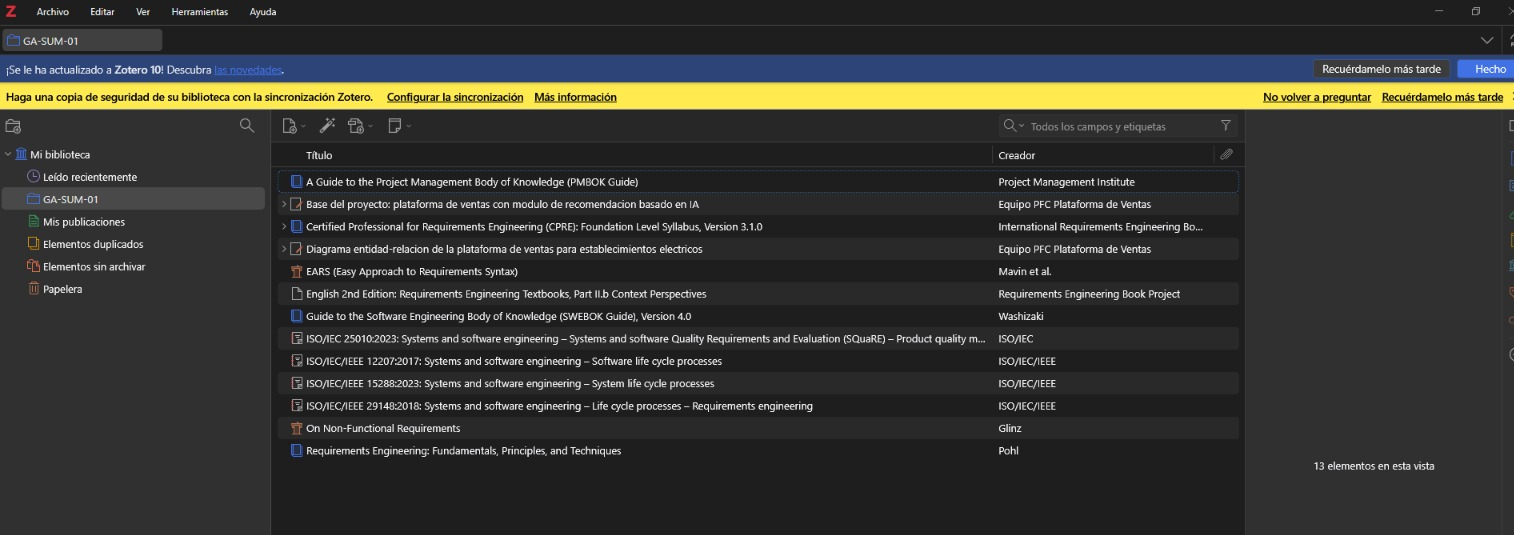
\includegraphics[width=0.99\textwidth]{figuras/captura_zotero_recorte.png}
\caption{Biblioteca Zotero de la práctica. Colección GA-SUM-01 con trece referencias registradas.}
\label{fig:zotero}
\end{figure}
\par\smallskip
\noindent\textbf{Alcance de los anexos.} El Anexo A documenta las referencias que figuraban en la biblioteca al realizar la exportación; la bibliografía del informe puede incorporar además artículos consultados posteriormente. Las actividades de campo, entrevistas y validaciones aún no realizadas no se presentan como resultados.
